\documentclass[a4paper,12pt]{report}

\usepackage{alltt, fancyvrb, url}
\usepackage{graphicx}
\usepackage[utf8]{inputenc}
\usepackage{float}
\usepackage{hyperref}
\usepackage[italian]{babel}
\usepackage{appendix}
\usepackage[italian]{cleveref}
\usepackage{xcolor}
\usepackage{microtype}
\usepackage{array}
\usepackage{adjustbox}
\usepackage{tabularx}
\usepackage{colortbl}
\usepackage{pdfpages}
\usepackage{listings}
\usepackage{booktabs}
\usepackage{longtable}
\usepackage{xltabular}
\usepackage{setspace}
\usepackage{ulem}
\usepackage{float}
\usepackage{tocloft}

\usepackage{natbib}
\bibliographystyle{plain}



\lstdefinestyle{codeStyle}{
    basicstyle=\small\ttfamily,
    keywordstyle=\color{blue},
    commentstyle=\color{green},
    stringstyle=\color{red},
    numbers=left,
    numberstyle=\tiny\color{gray},
    frame=single,
    breaklines=true,
    tabsize=2
}
\lstdefinestyle{pseudocode}{
    basicstyle=\ttfamily,
    keywordstyle=\color{blue}\bfseries,
    commentstyle=\color{gray}\itshape,
    stringstyle=\color{red},
    morekeywords={if, else, while, for, return, function, end, begin},
    morecomment=[l]{//},
    morecomment=[s]{/*}{*/},
    morestring=[b]",
	numbers=left,
    numberstyle=\tiny\color{gray},
    frame=single,
    breaklines=true,
    tabsize=2
}

\lstset{}
\newcolumntype{C}{>{\centering\arraybackslash}X}
\newcolumntype{D}{>{\center\arraybackslash}X}

\newcommand{\speciallabel}[2]{
	% \speciallabel{<stuff>}{<label>}
  \edef\@currentlabel{#1}\label{#2}%
}

\newcommand{\tableheader}{% % il comando prende quattro argomenti
\hline % disegna una linea orizzontale
\rowcolor{red} % colora la riga di rosso
\multicolumn{1}{|C|}{\textcolor{white}{\uppercase{concetto}}} & % centra e mette in grassetto il primo argomento
\multicolumn{1}{C|}{\textcolor{white}{\uppercase{costrutto}}} & % centra e mette in grassetto il secondo argomento
\multicolumn{1}{C|}{\textcolor{white}{\uppercase{accessi}}} & % centra e mette in grassetto il terzo argomento
\multicolumn{1}{C|}{\textcolor{white}{\uppercase{tipo}}} \\ % centra e mette in grassetto il quarto argomento
\hline % disegna una linea orizzontale
}

% A new counter for the rows
\newcounter{rowcntr}[table]
\renewcommand{\therowcntr}{\table\number\numexpr\value{rowcntr}\relax}


% A new columntype to apply automatic stepping
\newcolumntype{N}{>{\refstepcounter{rowcntr}\therowcntr}l}

% Reset the rowcntr counter at each new tabular
\AtBeginEnvironment{tabular}{\setcounter{rowcntr}{0}}

\setlength{\cftbeforesecskip}{0pt} % Riduce lo spazio verticale prima delle sezioni
\setlength{\cftaftertoctitleskip}{10pt} % Riduce lo spazio verticale dopo il titolo dell'indice

\graphicspath{{../resources/img}}
\title{\Large Course: Crittografia    \\[0.5cm]
        \bf\Large Crittografia applicata alla sicurezza di tutti i giorni: Bitwarden}
\author{\large Author: Edoardo Desiderio\\ \ \\}


\date{}

\begin{document}

	\makeatletter
		\begin{titlepage}
			\begin{center}
		{ 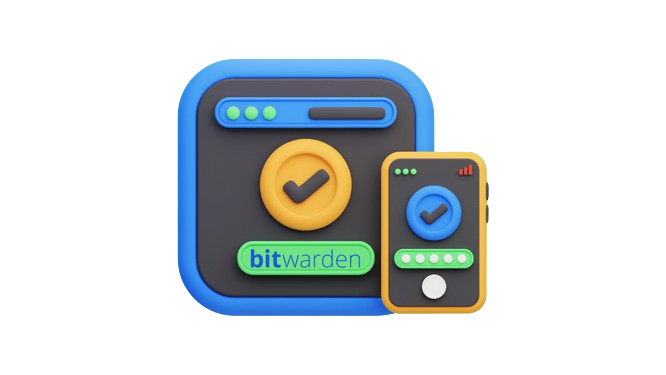
\includegraphics[width=10cm]{bitwarden-removebg-preview.png}}
		{\ \\}
			\vbox{}\vspace{2cm}
				{\@title }\\[3cm] 
				{\@author}
				{\large Instructor: \bf Prof. Luciano Margara\\ \ \\}
			\end{center}
		\end{titlepage}
	\makeatother
	\mbox{\thispagestyle{empty}}
	\titlepage
	\tableofcontents{\thispagestyle{empty}}
	\setcounter{page}{0}

	\chapter{Introduzione}
	\section{Scopo del Documento}
	L'idea della ricerca nasce poichè confrontandomi con amici e colleghi, ho notato
	che molti di loro studiavano il campo della crittografia da un punto di vista
	dei malware e dei ransomware, ma non da un punto di vista positivo. Questo
	documento ha lo scopo di fornire una panoramica generale della crittografia e
	delle sue applicazioni positive, con particolare attenzione ai password manager.
	\section{L'Uso Positivo della Crittografia} 
	La crittografia, un campo di studio che si
	occupa della protezione delle informazioni attraverso l'uso di codici, ha un
	ruolo fondamentale nel mondo digitale di oggi. Attraverso l'utilizzo di
	complessi algoritmi matematici, la crittografia protegge i dati sensibili,
	garantisce la riservatezza delle comunicazioni, assicura l'integrità dei dati e
	favorisce un commercio elettronico sicuro. È uno strumento cruciale per
	proteggere la nostra privacy e preservare la sicurezza dei nostri dati.
	La crittografia	è un elemento fondamentale per la cybersecurity, capace di assicurare una
	protezione efficace e duratura nel tempo dei sistemi e dei servizi a cui viene
	applicata. 
	\subsection*{Introduzione ai Password Manager} 
	Un password manager è un sistema di
	sicurezza informatica, un programma che permette di creare password uniche per
	ogni singolo account, conservarle in un luogo sicuro e accedere ad esse
	attraverso un’estensione del browser o una app, sia da un computer che da un
	dispositivo mobile come tablet o smartphone. Questi strumenti consentono agli
	utenti di sincronizzare le password tra vari dispositivi, e possono o meno
	conservare le password e i dati anche sul dispositivo.
	Il concetto principe di un password manager è quello di accedere
	ad una password unica, detta master password, che impastata
	rappresenta la chiave privata del mio storage di password.

	\section{Storia} 
	La storia dei password manager è intrinsecamente legata all'evoluzione della
	sicurezza informatica. Le password, come metodo di autenticazione, hanno radici
	antiche, risalenti all'antica Grecia e utilizzate per proteggere segreti
	militari durante la Seconda Guerra Mondiale. Con l'avvento dei computer negli
	anni '60, le password hanno iniziato a diventare parte della vita quotidiana.

	Il primo password manager della storia è stato sviluppato nel 1990 da Mark
	Thompson \cite{password-manager-hystory} e si chiama "password Safe" e 
	fu introdotto come software utility per windows 95. 

	\section{Passwword Save e l'algoritmo di Blowfish}
	Password Safe, nella sua versione originale, utilizzava l'algoritmo di
	crittografia \textbf{Blowfish} per proteggere le password memorizzate.
	Blowfish è un algoritmo di crittografia a blocchi simmetrico sviluppato da
	Bruce Schneier nel 1993.\\
	All'avvio, l'applicazione chiedeva all'utente di creare un nuovo archivio di
	password, che poteva essere salvato in qualsiasi posizione desiderata
	dall'utente. Dopo aver creato l'archivio, l'applicazione chiedeva all'utente di
	impostare una password principale. Questa password veniva utilizzata per
	bloccare l'accesso all'archivio delle password. Era l'unica password che
	l'utente doveva ricordare.\\
	Una volta impostata la password principale, l'utente poteva iniziare a
	memorizzare le proprie password e altre credenziali di accesso nell'archivio.
	Quando l'utente aveva bisogno di accedere alle sue password, doveva aprire
	l'applicazione Password Safe, inserire la password principale e quindi avrebbe
	avuto accesso all'archivio delle password.\\
	In questo modo, Password Safe offriva un modo sicuro per memorizzare tutte le
	password in un unico luogo, proteggendole con una sola password principale.
	Questo metodo di gestione delle password è ancora utilizzato nelle versioni più
	recenti di Password Safe e in molti altri gestori di password
	\subsection*{Punti chiave}
	\begin{itemize}
		\item \textbf{Crittografia Simmetrica:} Usa la stessa chiave\footnote{ la main password dell'utente} per
		crittografare e decrittografare i dati.
		\item \textbf{Lunghezza della Chiave Variabile:} Supporta chiavi di
		lunghezza variabile, da 32 a 448 bit, rendendolo flessibile in base alle
		esigenze di sicurezza.
		\item \textbf{Dimensione del Blocco:} Opera su blocchi di dati di 64
		bit.
		\item \textbf{S-Box:} Utilizza strutture interne note come
		S-box per realizzare la crittografia.
	\end{itemize}
	\newpage
	\section{Funzionamento di Blowfish}

	Blowfish utilizza un insieme di operazioni come sostituzioni e permutazioni,
	gestite attraverso S-box per trasformare il testo in chiaro in
	testo cifrato. Ogni blocco di dati viene elaborato in 16 round di
	crittografia.
	\begin{figure}[H]
		\centering
		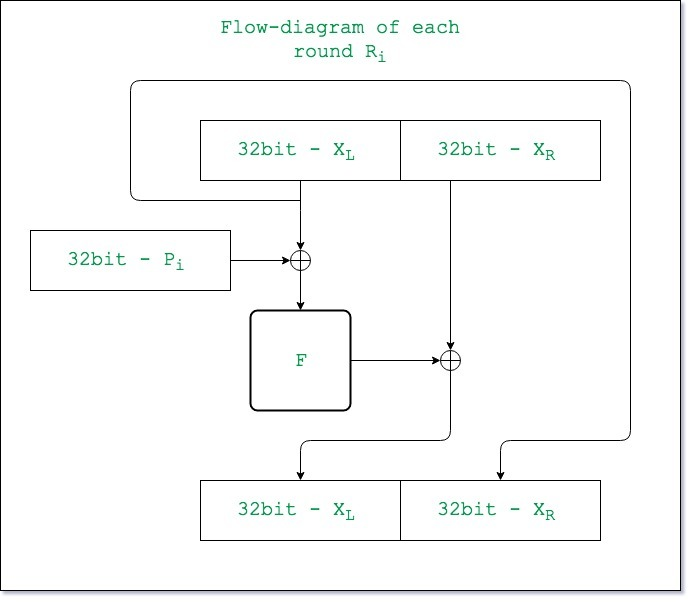
\includegraphics[width=0.9\textwidth]{encription.jpg}
		\caption{grafico che cattura il processo di crittografia dell'algoritmo \cite{blowfish-algorithm}}
		\label{fig:encription}
	\end{figure}


	\section*{Processo di Crittografia e Decrittografia}
	il processo principale di crittografia e decrittografia di Blowfish sta tutto 
	nella funzione \texttt{f} che utilizza le S-box per creare una funzione non
	lineare che contribuisce alla sicurezza dell'algoritmo.

	\begin{figure}[H]
		\centering
		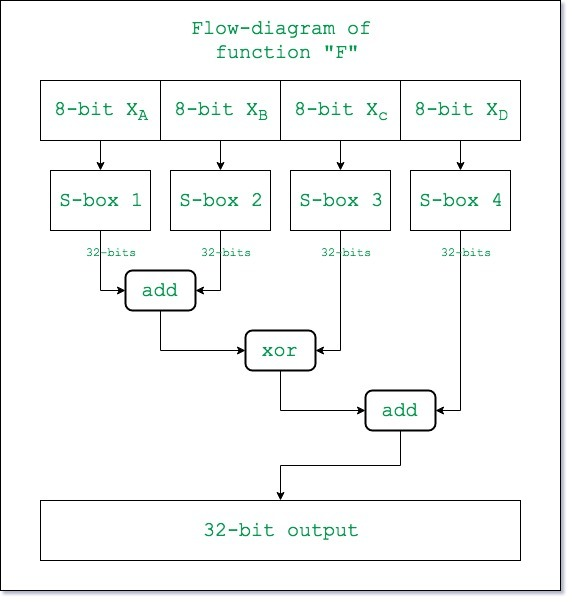
\includegraphics[width=0.9\textwidth]{F-blowfish.jpg}
		\caption{metodo f dell'algoritmo \cite{blowfish-algorithm}}
		\label{fig:f}
	\end{figure}
	% \begin{enumerate}
	% 	\item \textbf{Generazione delle S-Box :} Queste strutture
	% 	vengono inizializzate basandosi sulla chiave fornita dall'utente.
	% 	\item \textbf{Crittografia:} Il testo in chiaro viene diviso in blocchi
	% 	da 64 bit e ogni blocco viene processato attraverso le S-box
	% 	per produrre il testo cifrato.
	% 	\item \textbf{Decrittografia:} Avviene utilizzando la stessa chiave e
	% 	segue un processo simile alla crittografia, ma applicato in ordine
	% 	inverso.
	% \end{enumerate}
	\section*{Funzione $F$ dell'algoritmo Blowfish}

	La funzione $F$ prende in input un valore di 32 bit $x$ e restituisce un valore
	di 32 bit. Essa viene definita come segue:

	\[
		F(x) = ((S_1[a] + S_2[b] \bmod 2^{32}) \oplus S_3[c]) + S_4[d] \bmod 2^{32}
	\]
	\begin{itemize}
		\item $S_1, S_2, S_3, S_4$ sono le S-box dell'algoritmo.
		\item $a$ byte più significativo di x.
		\item $b$ = secondo byte più significativo di x
		\item $c$ = secondo byte meno significativo di x
		\item $d$ = byte meno significativo di x
		
	\end{itemize}
	
	\begin{lstlisting}[style=pseudocode]
		function F(x):
			result = ((S1[a] + S2[b] mod 2^32) xor S3[c]) + S4[d] mod 2^32
			
			return result
	\end{lstlisting}
	\section*{conclusioni sul funzionamento di Blowfish}
	in pratica l'algoritmo di crittografia Blowfish si differenzia
	principalmente dal DES visto a lezione per la sua chiave variabile fino a
	448 bit. \cite{blfh-lenth-key}

	\section*{L'obsolescenza di Blowfish nella prima versione di
	\textit{Password Safe}}

		
		Uno dei principali punti deboli di Blowfish risiede nella sua
		progettazione con una rete di Feistel di 16 round descritta nei
		paragrafi precedenti. Sebbene non vi siano attacchi pratici noti che
		possano rompere Blowfish con meno di 16 round, la struttura fissa e il
		numero limitato di round non garantiscono la stessa sicurezza di
		algoritmi più moderni come l'AES (Advanced Encryption Standard), che
		offre una configurazione più robusta e una gestione più sicura delle
		chiavi. Inoltre, la progettazione di Blowfish non è ottimizzata per le
		implementazioni hardware moderne, risultando vulnerabile a tecniche come
		gli attacchi \textit{time-memory trade-off} (TMTO) \footnote{Per
		maggiori informazioni sugli attacchi TMTO, si può consultare il seguente
		link:
		\url{https://en.wikipedia.org/wiki/Time/Memory/Data_Tradeoff_attack}} e
		l'utilizzo di tabelle precomputate.

		Con il tempo, la crittografia è diventata un campo in continua
		evoluzione, \par con attacchi sempre più sofisticati come quelli
		differenziali e lineari. Mentre Blowfish non è stato completamente
		compromesso da tali attacchi, la sua mancanza di aggiornamenti e
		adattamenti alle nuove minacce lo rende meno preferibile rispetto ad
		altri algoritmi che hanno subito una revisione continua e miglioramenti.\\

		Un'altra considerazione critica riguarda la derivazione\par delle chiavi. La
		prima versione di \textit{Password Safe} potrebbe non aver implementato
		meccanismi di derivazione delle chiavi robusti, come PBKDF2, bcrypt o
		Argon2, che sono progettati per resistere agli attacchi a forza bruta
		implementando salting e iterazioni multiple. Questo rende
		particolarmente problematico l'uso di Blowfish in contesti moderni, dove
		la sicurezza a lungo termine è essenziale.\\\\
		Inoltre, il supporto per chiavi di lunghezza fino a 448 bit, sebbene
		teoricamente sufficiente, non offre le stesse garanzie di sicurezza di
		AES con chiavi di lunghezza 256 bit, che è considerato lo standard di
		sicurezza per molte applicazioni critiche. La differenza non è solo
		nella lunghezza delle chiavi, ma anche nella resistenza agli attacchi,
		nella velocità di cifratura e nella versatilità in diversi ambienti
		hardware.e l'utilizzo di tabelle precomputate.\\\\
		Un'altra considerazione critica riguarda la derivazione delle chiavi. La prima
		versione di \textit{Password Safe} potrebbe non aver implementato meccanismi di
		derivazione delle chiavi robusti, come PBKDF2, bcrypt o Argon2, che sono
		progettati per resistere agli attacchi a forza bruta implementando salting e
		iterazioni multiple. Questo rende particolarmente problematico l'uso di Blowfish
		in contesti moderni, dove la sicurezza a lungo termine è essenziale.\\
		Inoltre, il supporto per chiavi di lunghezza fino a 448 bit, sebbene
		teoricamente sufficiente, non offre le stesse garanzie di sicurezza di AES con
		chiavi di lunghezza 256 bit, che è considerato lo standard di sicurezza per
		molte applicazioni critiche. La differenza non è solo nella lunghezza delle
		chiavi, ma anche nella resistenza agli attacchi, nella velocità di cifratura e
		nella versatilità in diversi ambienti hardware.

		\chapter{Bitwarden}
		\section{Introduzione}
		\sloppy Bitwarden è un password manager open source che offre una soluzione sicura
		per memorizzare e gestire le password. È disponibile su diverse piattaforme,
		tra cui desktop, web, mobile e browser. Bitwarden offre funzionalità di
		sincronizzazione, condivisione e generazione di password, nonché un'interfaccia
		intuitiva e facile da usare.\\
		
		\begin{figure}[H]
			\centering
			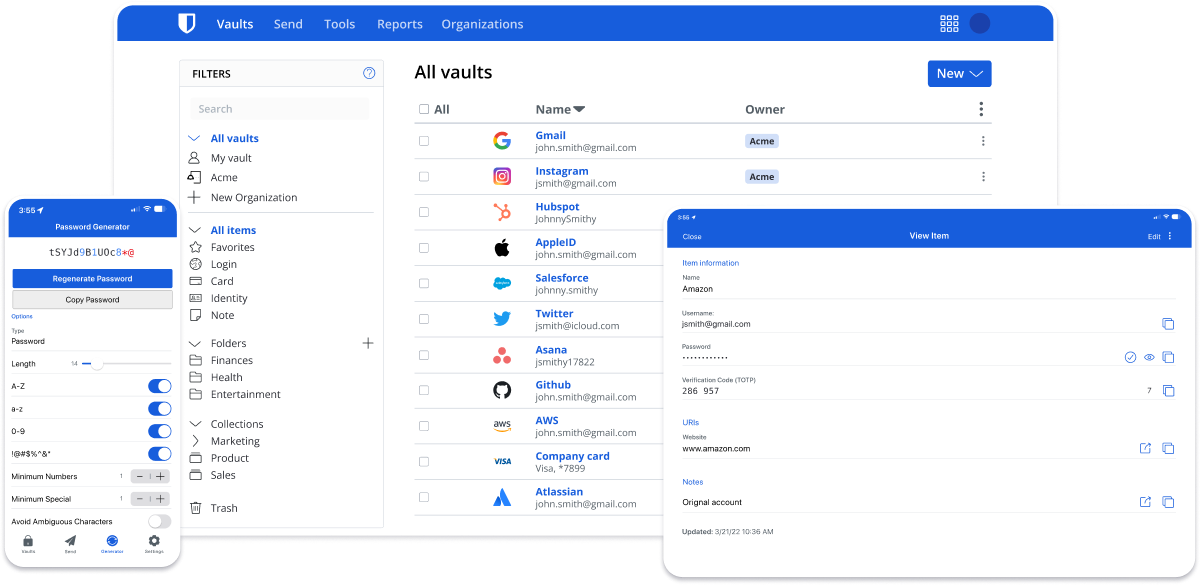
\includegraphics[width=0.9\textwidth]{wardenEnviroment.png}
			\caption{l'enviroment di Bitwarden}
			\label{fig:eviroment}
		\end{figure}

		\section{missione del progetto}
		Bitwarden è un progetto open source che si pone l'obiettivo di \\
		fornire
		una soluzione sicura e affidabile per la gestione delle password. La
		missione di Bitwarden è quella di proteggere la privacy e la sicurezza
		degli utenti, offrendo un servizio gratuito e open source che garantisce
		la riservatezza dei dati e la sicurezza delle informazioni personali.
		Rendendo il suo codice \href{https://github.com/bitwarden}{sorgente}
		pubblico nel 2016, Bitwarden ha dimostrato il suo impegno per la
		trasparenza e la sicurezza, consentendo agli utenti di verificare la
		qualità del software e la sicurezza delle loro password.\\
		
		


	\newpage
	\bibliography{refs}
	\renewcommand{\bibsection}{}
	\chapter*{Riferimenti bibliografici}
	
\end{document}
